\chapter{Pruebas}

Las pruebas realizadas en RSMap han supuesto cambios mínimos sobre los que se ha ido mejorando lo anterior por lo que no se tiene una perspectiva completa de todos las pruebas realizadas ya que serían cientos, sin embargo el conjunto de esos pequeños cambios se puede agrupar en problemas a los cuales se le ha encontrao una solución en la mayoría de los casos.
\bigskip

Se ha monitorizado la carga que sufren los servidores cuando se encuentra sometidos a trabajo. Debido a que Amazon EC2 proporciona un sistema autoescalable, éste aspecto no es de gran preocupación. No obstante los resultados obtenios indican que la aplicación RSMap en su cojunto no supone un gran coste de recursos como podemos ver en las siguientes imágenes:

\begin{figure}[ht]
  \begin{center}
    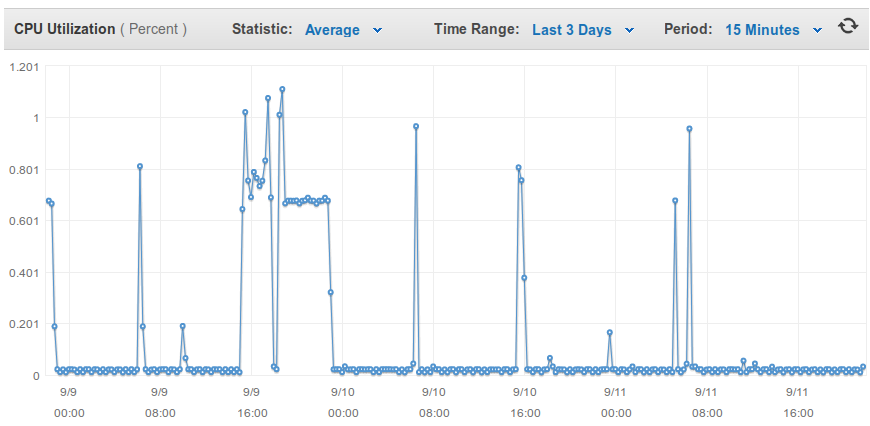
\includegraphics[scale=0.40]{../images/amazon/cpuweb.png}
    \caption{Carga CPU del servidor web y API}
    \label{fig:paquetes}
  \end{center}
\end{figure}

\newpage

\begin{figure}[ht]
  \begin{center}
    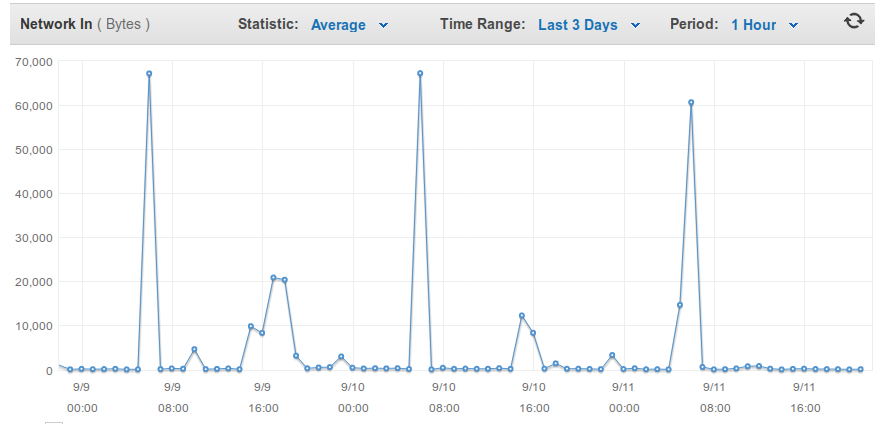
\includegraphics[scale=0.40]{../images/amazon/netweb.png}
    \caption{Carga de entrada de red del servidor web y API}
    \label{fig:paquetes}
  \end{center}
\end{figure}

\begin{figure}[ht]
  \begin{center}
    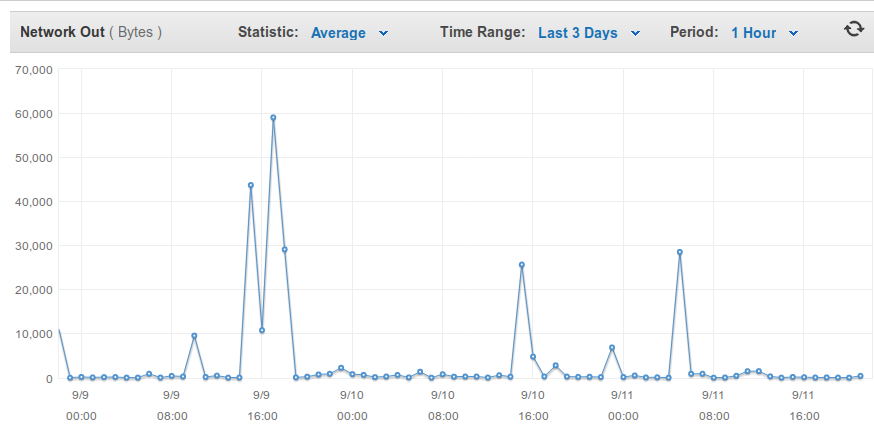
\includegraphics[scale=0.40]{../images/amazon/netwebou.png}
    \caption{Carga de salida de red del servidor web y API}
    \label{fig:paquetes}
  \end{center}
\end{figure}

\newpage

\begin{figure}[ht]
  \begin{center}
    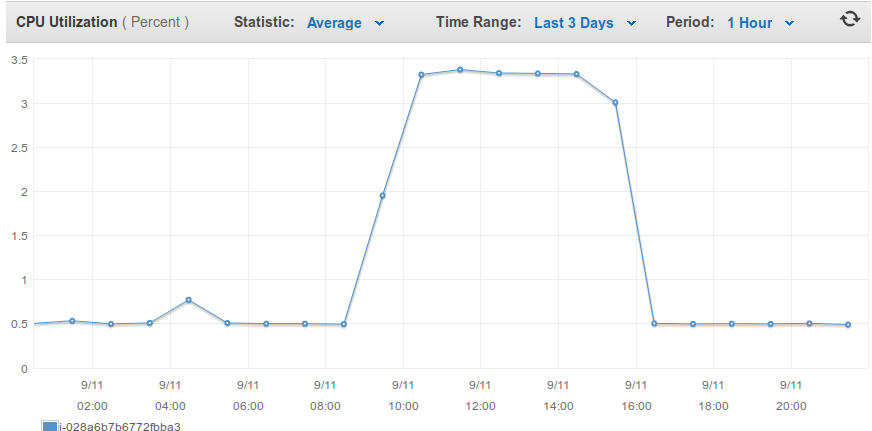
\includegraphics[scale=0.40]{../images/amazon/cpucassandra.png}
    \caption{Carga CPU del servidor de Cassandra}
    \label{fig:paquetes}
  \end{center}
\end{figure}

\begin{figure}[ht]
  \begin{center}
    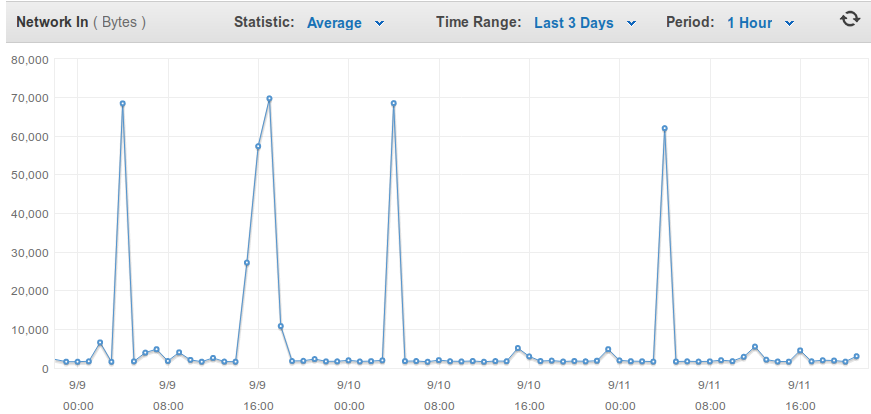
\includegraphics[scale=0.40]{../images/amazon/netcassandra.png}
    \caption{Carga de entrada de red del servidor de Cassandra}
    \label{fig:paquetes}
  \end{center}
\end{figure}

\newpage

\begin{figure}[ht]
  \begin{center}
    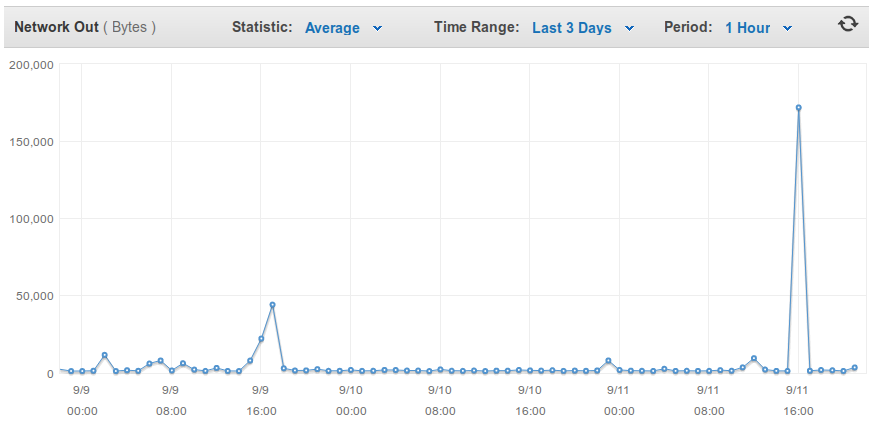
\includegraphics[scale=0.40]{../images/amazon/netcassandraou.png}
    \caption{Carga de salida de red del servidor de Cassandra}
    \label{fig:paquetes}
  \end{center}
\end{figure}

\begin{figure}[ht]
  \begin{center}
    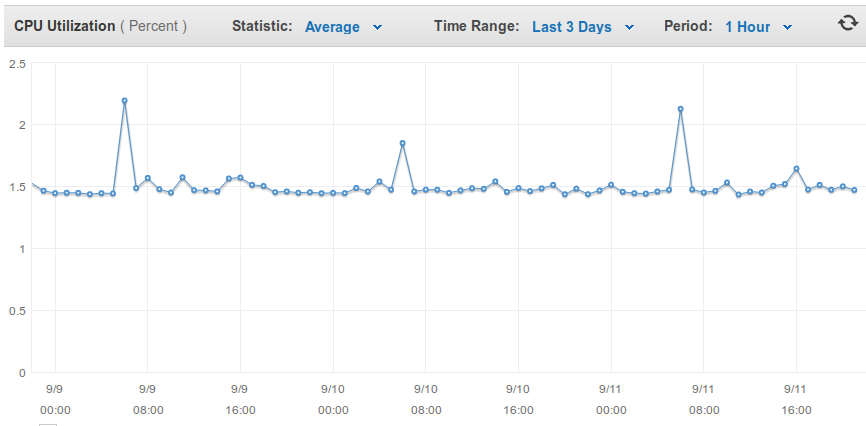
\includegraphics[scale=0.40]{../images/amazon/cpuzepp.png}
    \caption{Carga CPU del servidor de Zeppelin }
    \label{fig:paquetes}
  \end{center}
\end{figure}

\newpage

\begin{figure}[ht]
  \begin{center}
    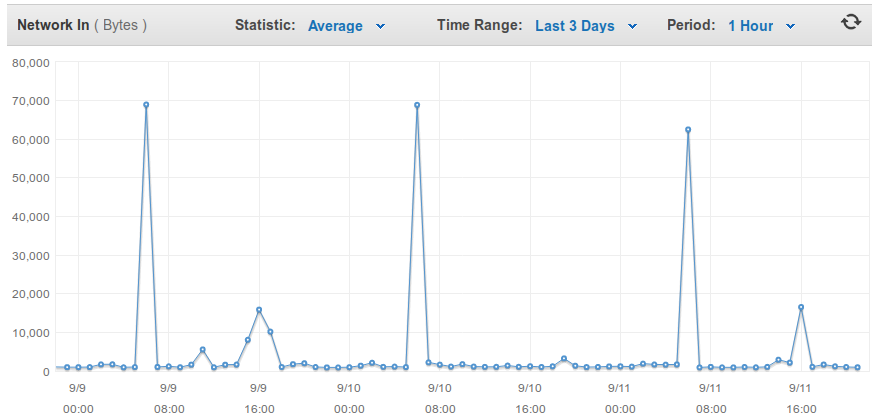
\includegraphics[scale=0.40]{../images/amazon/netzepp.png}
    \caption{Carga de entrada de red del servidor de Zeppelin}
    \label{fig:paquetes}
  \end{center}
\end{figure}

\begin{figure}[ht]
  \begin{center}
    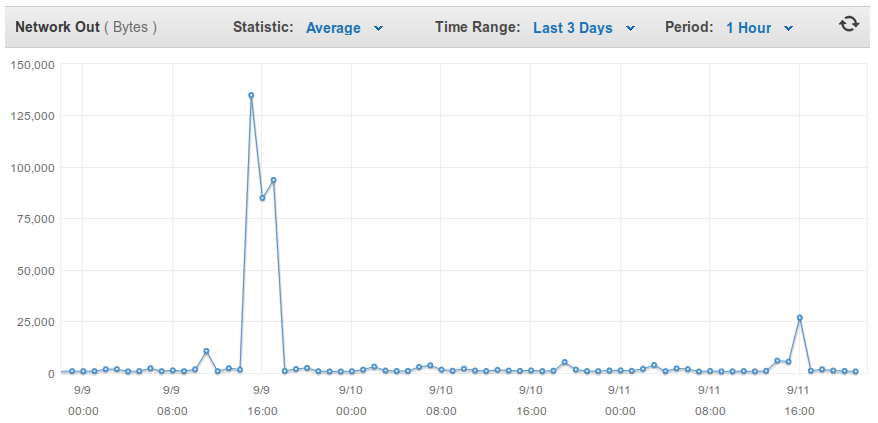
\includegraphics[scale=0.40]{../images/amazon/netzeppou.png}
    \caption{Carga de salida de red del servidor de Zeppelin}
    \label{fig:paquetes}
  \end{center}
\end{figure}

\newpage

El dispositivo receptor Raspberry Pi ha demostrado haber sido una elección correcta ya que en ningún momento se ha presentado algún problema relacionado con el rendimiento, es más, los recursos usados cuando la aplicación está funcionano no superan un 30\% del total por lo que éste dispositivo tiene cabida para actividades computacionalmente mucho más complejas de las que se han llevado a cabo finalmente.

\bigskip

La siguiente tabla muestra las fases críticas en el desarrollo, configuración y construcción del proyecto y los errores y soluciones que se han propuesto para combatirlos.

\newpage

\begin{table}[!h]
\centering
\label{my-label}
\begin{tabular}{llll}
\hline
\multicolumn{1}{|l|}{Nombre} & \multicolumn{1}{l|}{Descripción} & \multicolumn{1}{l|}{Resultado} & \multicolumn{1}{l|}{Solución} \\ \hline
P1 & \begin{tabular}[c]{@{}l@{}}Conexión con la \\ tarjeta de sonido\end{tabular} & OK &  \\ \hline
P2 & \begin{tabular}[c]{@{}l@{}}Obtención de \\ valores que \\ representen\\ el sonido obtenido\end{tabular} & OK &  \\ \hline
P3 & \begin{tabular}[c]{@{}l@{}}Comunicación\\ entre hebras\end{tabular} & OK &  \\ \hline
P4 & \begin{tabular}[c]{@{}l@{}}Identificación de\\ vehículos\end{tabular} & OK &  \\ \hline
P5 & \begin{tabular}[c]{@{}l@{}}Generación de\\ SDK en KAA\end{tabular} & OK &  \\ \hline
P6 & \begin{tabular}[c]{@{}l@{}}Comunicación\\ entre Python y Java\end{tabular} & \begin{tabular}[c]{@{}l@{}}No se pudo creando\\ un subproceso\\ desde Python.\end{tabular} & \begin{tabular}[c]{@{}l@{}}Crear un Socket\\ en Java.\end{tabular} \\ \hline
P7 & \begin{tabular}[c]{@{}l@{}}Integración\\ entre Java y KAA\\ SDK\end{tabular} & OK &  \\ \hline
P8 & \begin{tabular}[c]{@{}l@{}}Envío de datos\\ a Cassandra\end{tabular} & ERROR & \begin{tabular}[c]{@{}l@{}}Abrir los\\ puertos correctos.\end{tabular} \\ \hline
P9 & \begin{tabular}[c]{@{}l@{}}Uso de Scala para\\ definir las de tiempo\\ en Zeppelin\end{tabular} & ERROR & \begin{tabular}[c]{@{}l@{}}Definir las funciones\\ dentro de Cassandra,\\ en Java.\end{tabular} \\ \hline
P10 & \begin{tabular}[c]{@{}l@{}}Conexión de Zeppelin\\ y Cassandra\end{tabular} & OK &  \\ \hline
P11 & \begin{tabular}[c]{@{}l@{}}Consultas en\\ Cassandra\end{tabular} & ERROR & \begin{tabular}[c]{@{}l@{}}Corregir el esquema\\ de datos definido\\ en Cassandra\end{tabular} \\ \hline
P12 & \begin{tabular}[c]{@{}l@{}}Escritura mediante\\ rutas en la API\end{tabular} & OK &  \\ \hline
P13 & \begin{tabular}[c]{@{}l@{}}Lectura mediante\\ rutas de la API\end{tabular} & OK &  \\ \hline
P14 & \begin{tabular}[c]{@{}l@{}}Actualización\\ mediante \\ rutas de la API\end{tabular} & ERROR & \begin{tabular}[c]{@{}l@{}}El método a usar\\ es PATCH y no PUT.\end{tabular} \\ \hline
P15 & \begin{tabular}[c]{@{}l@{}}Eliminación mediante\\ rutas de la API\end{tabular} & OK &  \\ \hline
P16 & \begin{tabular}[c]{@{}l@{}}Chequeo de tiempos\\ de las señales\\ recibidas\end{tabular} & OK &  \\ \hline
P17 & \begin{tabular}[c]{@{}l@{}}Diseño responsive \\ en la web\end{tabular} & \begin{tabular}[c]{@{}l@{}}ERROR, Para web y tablets\\ tiene una correcta\\ visualización, para\\ smartphones el mapa\\ se redimensiona\\ incorrectamente.\end{tabular} & No solucionado. \\ \hline
\end{tabular}
\caption{Pruebas realizadas sobre RSMap}
\end{table}
